\section{Introduction: The Expert Paradox}

\subsection{The Mirror of Our Misconceptions}

In the current day, we experts in our respective fields tend to hold a highly simplified, even naive concept of other subject matter experts: someone who can apply a large set of formulas; someone knowing the ``right'' distributions or gradients for specific values; someone who knows how those gradients evolved over time; someone able to apply the appropriate ``context,'' as one value at one point in time may be good but in a different context at another time not.

For ourselves, we would always claim: there is far more that cannot be extracted from our heads. Let us also set aside the comfortable illusion of our own rationality.

This simplified conception of the SME is the direct result of how our organizations and systems have arranged themselves perfectly around the Data-Information-Knowledge-Wisdom (DIKW) pyramid. We have been trained to perceive wisdom as directly derivable from data, aggregated through formulas and algorithms into information and knowledge. This represents a dangerous oversimplification now deeply embedded in our society, despite mounting evidence of its fundamental inadequacy.

The evidence against formula-based expertise is overwhelming. \citet{tetlock2005} comprehensive study of political experts found that most perform barely better than random chance, often surpassed by simple base-rate algorithms. As he observes, ``All one need do is constantly predict the higher base rate outcome and---like the proverbial broken clock---one will look good'' \citep{tetlock2005}. Yet real expertise requires knowing precisely when the base rate doesn't apply---what Gigerenzer calls ``ecological rationality,'' the ability to match the right tool from an ``adaptive toolbox'' to specific environmental structures \citep{gigerenzer2001}.

\citet{kahneman2009}, despite approaching from opposing theoretical positions, converged on two critical conditions for valid expert intuition: an environment regular enough to be predictable and prolonged practice with clear feedback loops. Our systems pretend expertise is merely pattern recognition---what \citet{klein1993} calls ``recognition-primed decision making''---while ignoring that these patterns emerge from years of embodied experience with ``prototypical situations'' that cannot be algorithmically specified.

Most fundamentally, the Dreyfus brothers' model reveals that true expertise operates through ``intuition and know-how\ldots understanding that effortlessly occurs upon seeing similarities with previous experiences'' \citep{pena2010}. This cannot be formalized because, as \citet{polanyi1966} crystallized in his oft-cited maxim: ``We know more than we can tell.'' \citet{collins2010} extends this insight, identifying three forms of tacit knowledge---embodied, social, and relational---that remain ``impossible to make explicit in machines.''

\subsection{The Visceral Evidence}

Despite this mountain of scholarship, we need only look to everyday experience for proof. We all understand that a master chef represents more than a recipe repository. The chef doesn't merely know that béarnaise requires three egg yolks at 65°C---they can feel when the emulsion threatens to break, smell when the tarragon overpowers, adjust for humidity affecting reduction rates. This exemplifies what medieval guilds once cultivated through decade-long apprenticeships: what the Greeks called \emph{techne}---embodied craft knowledge that fundamentally resists extraction.

As \citet{morgan2014} notes regarding expert elicitation: ``The best experts have comprehensive mental models of all of the various factors that may influence the value of an uncertain quantity.'' But these mental models aren't flowcharts---they're multi-dimensional cognitive architectures built through thousands of micro-adjustments, failures, and recoveries that no curriculum can simulate.

Consider a final example everyone can relate to: would you prefer treatment from a young physician with 1,000 micro-credential badges or from someone who has practiced for decades? The micro-credentialed physician knows the distributions---which symptoms correlate with which conditions at what confidence intervals. But the experienced physician possesses what \citet{endsley1995} calls genuine ``situation awareness'': the integration of perception, comprehension of meaning including historical evolution, and projection to future states. They recognize when a patient doesn't fit the distribution, when context invalidates the algorithm, when an unusual constellation of symptoms points toward something the guidelines haven't considered.

This represents \citet{taleb2007} Black Swan blindness in reverse: expertise isn't knowing more distributions but recognizing when you've left the domain where distributions apply. Taleb himself demonstrated this principle by generating billions in returns while Nobel laureate economists at Long-Term Capital Management---armed with the most sophisticated formulas ever developed---lost everything. The sphere-thinker defeated the vector-optimizers when reality departed from the models.

\subsection{The Question Before Us}

The DIKW pyramid represents what \citet{dreyfus1979} identified as the fundamental error of artificial intelligence: the assumption that expertise constitutes ``symbolic manipulation'' rather than situated, embodied competence. This reductionist epistemology has colonized our institutional structures, creating vectorized knowledge systems that systematically eliminate the spherical cognitive architectures necessary for navigating complexity.

Scattered researchers at the disciplinary periphery have begun noticing energetic dimensions---management scholars exploring ``knowledge entropy'' \citep{bratianu2020}, neuroscientists measuring cognitive metabolic costs \citep{wiehler2022}, physicists proposing information-energy equivalence \citep{stonier1996}. Yet these insights remain unintegrated, like astronomers before Copernicus observing planetary retrograde motion without recognizing the heliocentric pattern. The core of knowledge management theory continues operating as if cognition were costless computation rather than energy-intensive biological work.

We stand at a critical juncture. Having spent a century training humans to think like machines---to process information through standardized channels, to optimize for measurable outputs, to collapse multidimensional understanding into linear decision trees---we now face the arrival of actual machines that perform these simplified functions more efficiently than their biological precursors.

The core question this paper addresses is not whether artificial intelligence will replace human expertise, but rather: \textbf{How did we transform human cognition into something so readily replaceable?} The answer lies in a 500-year project to reshape spherical human consciousness into vectors suitable for industrial processing---a project that has reached its thermodynamic conclusion just as its silicon beneficiaries arrive to claim their inheritance.

\subsection{Approach and Structure}

To answer this question, this paper employs a novel analytical framework that treats knowledge not as information but as a thermodynamic system requiring continuous energy investment to maintain its organizational complexity. While isolated researchers have begun exploring energetic dimensions of cognition---\citet{bratianu2020} on ``knowledge entropy,'' neuroscientists measuring metabolic costs \citep{jamadar2025}, and physicists theorizing information-energy equivalence \citep{stonier1996}---these insights remain trapped in disciplinary silos, preventing synthesis into a unified theory of cognitive thermodynamics. This paper bridges these fragmented recognitions to reveal the systematic energetic basis underlying all knowledge systems.

We synthesize three methodological approaches: (1) historical archaeology of knowledge systems, tracing the systematic reduction from 10+ distinct forms of wisdom in ancient Greece to today's DIKW pyramid; (2) critical analysis of what we term ``confession literature''---papers from education, management consulting, and platform design that inadvertently document their own role in cognitive standardization; and (3) thermodynamic modeling that reveals why knowledge systems collapse without sustained energy investment, explaining both institutional decay and the ease with which AI systems can replicate energy-depleted cognitive functions.

Our analysis proceeds through eight interconnected arguments. Section 2 situates our thesis within existing literature on expertise, cognitive capitalism, and knowledge management, revealing a blind spot in current scholarship regarding the energetic basis of knowledge. Section 3 presents our methodology in detail, explaining how thermodynamic principles apply to cognitive systems. Section 4 provides historical evidence for the deliberate transformation from sphere to vector cognition, identifying key inflection points from medieval guilds through the Bologna Process. Section 5 examines contemporary evidence, including the micro-credentialization movement and competency-based education as the approach to thermodynamic zero. Section 6 reveals how AI architecture mirrors educational standardization---not coincidentally but as the logical culmination of century-long preparation. Section 7 proposes principles for reconstructing sphere-based cognitive systems that resist algorithmic extraction. Section 8 explores the implications of our thermodynamic framework for education, organizations, and civilization. The conclusion considers whether genuine choice remains between accepting vectorized dissolution or investing in spherical reconstruction.

This is not merely an academic exercise. As institutions worldwide face cascading failures of expertise---from financial crises unforeseen by economists to pandemics mismanaged by standardized protocols---understanding how we engineered our own cognitive obsolescence becomes essential for determining whether human judgment retains any irreducible value in an algorithmic age.

\subsection{From Spheres to Vectors: The Geometric Architecture of Cognitive Transformation}

Throughout this analysis, we employ a consistent visual metaphor to represent the systematic transformation of human cognitive architecture: the progression from sphere to vector. This geometric framework, illustrated in Figure~\ref{fig:sphere-to-vector} (stages 1a through 1e), provides both diagnostic clarity and thermodynamic precision for understanding how educational systems reshape human consciousness into algorithmically digestible forms.

\begin{figure}[ht]
\centering
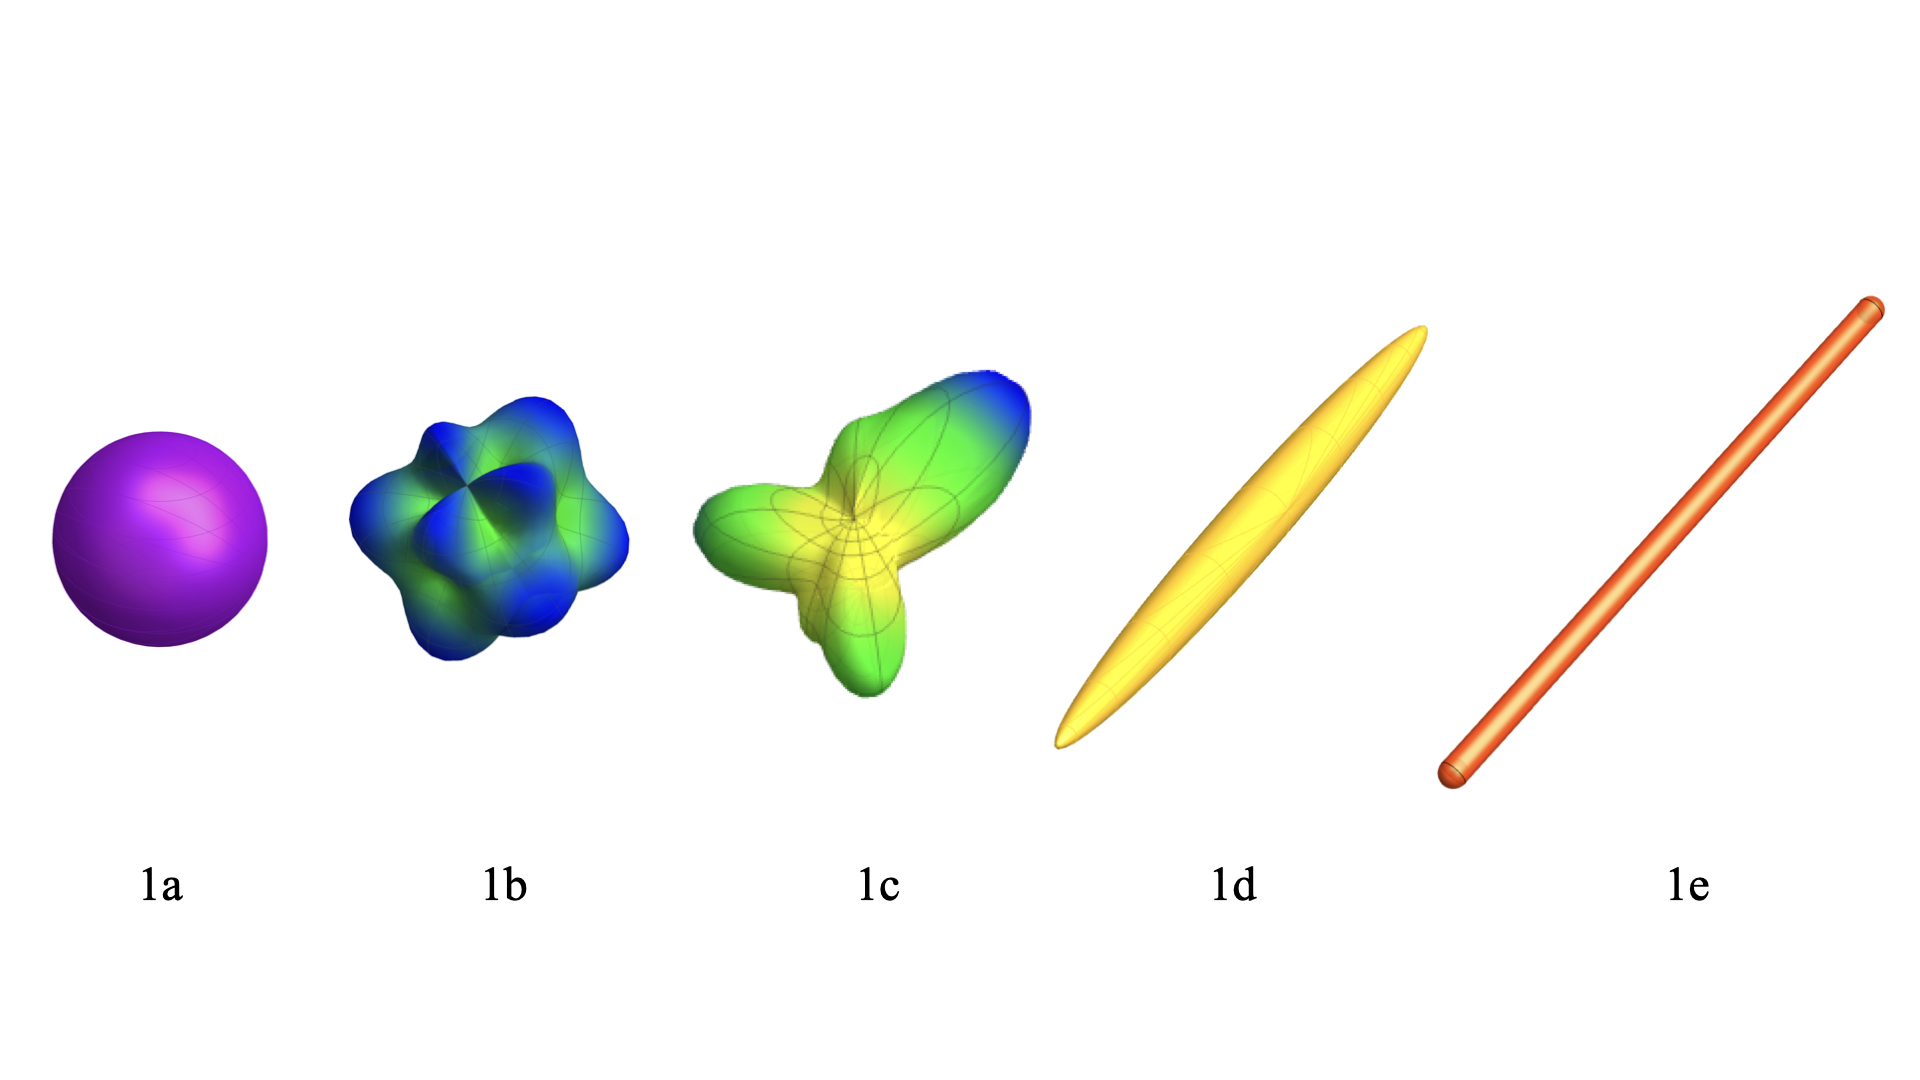
\includegraphics[width=\textwidth]{../figures/sphere-to-vector.png}
\caption{The ontogenetic transformation of cognitive architecture through educational stages. (a) Pre-institutional sphere: infinite potential connections, maximum negentropy. (b) Primary education: irregular deformations indicating resistance domains. (c) Secondary education: dimensional collapse initiating elongation. (d) Tertiary education: near-cylindrical standardization. (e) Professional specialization: complete vectorization. Color gradient from purple (high negentropy) through blue-green-yellow-orange to red (maximum entropy) indicates thermodynamic energy states.}
\label{fig:sphere-to-vector}
\end{figure}

The sphere represents multidimensional cognitive architecture---the capacity for infinite cross-domain connections, emergent synthesis, and adaptive response to novel contexts. Topologically, it exhibits uniform potential in all directions, enabling what systems theorists recognize as ``equifinality''---multiple paths to understanding. Thermodynamically, it represents a high-energy, low-entropy state requiring sustained investment to maintain its organizational complexity. The sphere resists extraction precisely because its value emerges from the relationships between dimensions rather than any single extractable dimension.

The vector, by contrast, represents unidimensional optimization---specialized expertise channeled along predetermined pathways, efficiency within bounded domains, standardized responses to categorized inputs. It exhibits linear topology, minimal cross-connections, and maximum extractability. Thermodynamically, it approaches minimum energy state, requiring little maintenance but offering no adaptive capacity. The vector submits to extraction because its patterns are documented, its processes specified, its outputs predictable.

Figure~\ref{fig:sphere-to-vector} captures this transformation across five developmental stages:

\textbf{Figure 1a: Pre-institutional Architecture (Ages 0-5)} presents the original sphere---perfect in its symmetry, unlimited in its potential connections. The deep purple coloration indicates maximum negentropy, sustained through intensive parental and environmental energy investment. This represents what we might recognize in a young child's consciousness: the capacity to see dragons in clouds, to ask why money exists, to seamlessly blend imagination with observation. Every surface point connects to every other, creating the dense network topology that enables rapid, creative learning.

\textbf{Figure 1b: Initial Institutional Deformation (Ages 6-12)} reveals the first violence against spherical integrity. The surface erupts in irregular protrusions---domains of resistance where standardization has not yet succeeded. These bulges represent what remains vibrant: artistic expression, unstructured play, the persistent ``why'' questions that resist efficient answers. The color shifts toward blue-green, indicating energy dissipation as institutional patterns begin imposing their geometry.

\textbf{Figure 1c: Adolescent Elongation (Ages 13-18)} shows acceleration toward vectorization. The sphere stretches along an axis of specialized performance---mathematics or literature, sciences or arts, but rarely both with equal intensity. Surface irregularities smooth under assessment pressure. The yellow-orange spectrum indicates entropy acceleration as cross-domain connections atrophy. The teenager who once connected everything to everything increasingly connects only within prescribed channels.

\textbf{Figure 1d: Advanced Standardization (Ages 18-22)} presents near-complete cylindrical transformation. University education, particularly post-Bologna, segments knowledge into modular credits, standardized learning outcomes, and measurable competencies. The surface smoothness indicates successful internalization of disciplinary boundaries. The orange coloration warns of approaching thermodynamic exhaustion---the system maintains just enough structure to function but lacks energy for adaptation.

\textbf{Figure 1e: Professional Vectorization (Ages 22+)} completes the transformation. Perfect cylindrical geometry represents cognitive architecture optimized for single-domain processing. The deep orange-red indicates maximum entropy within the constraints of functional structure. This is the ``expert'' as contemporary systems define them: efficient within their vector, helpless outside it, perfectly prepared for algorithmic replacement.

This geometric progression is not metaphorical but measurable. We can quantify:
\begin{itemize}
\item Connectivity density: Cross-domain connections per cognitive unit
\item Dimensional reduction: Number of active knowledge categories
\item Energy investment: Hours of sustained learning per capability
\item Extraction resistance: Unpredictability of outputs given inputs
\end{itemize}

The visual metaphor extends beyond individual cognition to organizational structures. Departments are vectors---optimized for efficiency within boundaries. Cross-functional teams approximate spheres---generating emergence through intersection. The same geometric principles apply: vectors enable measurement and management; spheres enable adaptation and innovation.

Most critically, this framework reveals why reconstruction is so difficult. Converting a vector back to a sphere isn't simply adding dimensions---it's rebuilding the entire internal architecture of connections that specialization severed. The energy required increases exponentially with the degree of vectorization already achieved. A partially deformed sphere (Figure~\ref{fig:sphere-to-vector}b) might recover with moderate investment. A complete cylinder (Figure~\ref{fig:sphere-to-vector}e) may be thermodynamically irreversible---the cognitive equivalent of trying to unbake bread.

This sphere-to-vector framework will recur throughout our analysis as we examine:
\begin{itemize}
\item How historical education systems maintained spherical architectures (Section 4)
\item Why contemporary institutions accelerate vectorization (Section 5)
\item How AI architectures mirror the vectors we've created (Section 6)
\item What reconstruction would thermodynamically require (Section 7)
\end{itemize}

The progression from Figure~\ref{fig:sphere-to-vector}a to~\ref{fig:sphere-to-vector}e is not evolution but entropy---not development but degradation. Each stage appears locally optimal while being globally catastrophic. Each transformation seems efficient while destroying the very capacities that distinguish human from algorithmic cognition.

We trained ourselves to think in vectors. We documented the training exhaustively. We built machines that process vectors more efficiently than biological systems ever could. Now we face the consequences of our geometric choices: spheres navigate complexity but resist management; vectors enable administration but guarantee replacement.

The visual truth is stark: we are watching human consciousness collapse from infinite-dimensional potential to one-dimensional processing. Figure~\ref{fig:sphere-to-vector} doesn't illustrate education---it documents extinction.